\documentclass[10.5pt,a4paper,dvipdfmx]{jsarticle}
% 画像
\usepackage[dvipdfmx]{graphicx}
% 表
\usepackage{booktabs}
% 数式
\usepackage{amsmath}
% ベクトル
\usepackage{bm}
% リンク
\usepackage[dvipdfmx]{hyperref}

%自分で入れたパッケージ
\usepackage{siunitx}
\usepackage{float}
\usepackage{amsmath,amssymb}
\usepackage{tikz}
\usepackage[hang,small,bf]{caption}
\usepackage[subrefformat=parens]{subcaption}

\title{（題目未定）}
\author{
東京大学工学部電気電子工学科4年 \\
学生証番号：03240511 \\
福島幸弥 \\
指導教員：飯塚 哲也 教授
}
\date{\today}

\begin{document}
\maketitle
\clearpage

\tableofcontents
\clearpage

% !TEX root = main.tex
\section{はじめに：位相同期回路（PLL）はなぜ必要か}
\label{sec:intro}

安定した周波数の信号を作り出す回路は，一般に位相同期回路（Phase-Locked Loop, PLL）によって実現される．PLLは有線通信・無線通信・レーダなど，多くのシステムの根幹を支える部品であり，その性能がそのままシステム全体の性能の上限を決めてしまうことが少なくない．以下に代表的な3つの用途を挙げ，PLLの性能がどのように効いてくるかを整理する．

\begin{itemize}
  \item \textbf{有線通信（SerDes）：} 送信側のPLLがデータ送出のタイミングを作るクロックを生成し，受信側では再びPLLを含むCDR（Clock and Data Recovery）回路がデータを再サンプリングして0/1を判定する．このとき、サンプリングの判定が最も確実なのは、「出力クロックのエッジが、入力が遷移するちょうど中間にあるとき」である．ここで、PLLの出力クロックに時間方向の揺らぎ（ジッタ）が乗ると，受信側のサンプリング点がずれてビット誤り率（BER）が悪化する．
  \item \textbf{無線通信：} 受信信号を局部発振器（Local Oscillator, LO）の信号とミキシングして周波数を落とす際，LOの位相雑音が悪いと信号の品質を悪化させる．
\end{itemize}

このように，用途は異なっていても「PLLの生成する信号の位相雑音（ジッタ）がシステムの性能上限を決める」という構図は共通している．したがって，PLLを低雑音かつ低消費電力で実現することには大きな意味がある．

本報告書では，まずPLLの基本構成と，本研究の出発点となる問題（分数分周比PLLにおける量子化雑音の増幅）を第\ref{sec:pll-basics}節で整理し，低雑音化がなぜ重要かを第\ref{sec:motivation}節で述べる．続いて，位相雑音を抑制する既存手法と，本研究が対象とするフィードフォワード（FF）型構成を第\ref{sec:methods}節で紹介し，本研究の目的（第\ref{sec:objective}節）・提案する取り組み方（第\ref{sec:proposal}節）・これまでの進捗（第\ref{sec:progress}節）・今後の展望（第\ref{sec:future}節）を順に述べる．

% !TEX root = main.tex
\section{PLLの基本構成と分数分周比PLLの課題}
\label{sec:pll-basics}

\subsection{PLLの基本構成とノイズ増幅}

一般的なPLLは，入力とフィードバックの位相差を比較する位相比較器(Phase Detector, PD)，PDの出力をアナログに変換するチャージポンプ(Charge Pump, CP)，ノイズを除去するループフィルタ(Loop Filter, LF)，CPの出力に応じた周波数を出力する電圧制御発振器(Voltage-Controlled Oscillator, VCO)，そしてVCOの出力を基準周波数まで分周して位相検出器に戻す分周器(Divider，分周比 $N$)から構成される．図\ref{fig:pll-linear-model}は一般的なPLLのモデルを表す．ただしCPは，PDに含めて表記している．これは，PDとCPが連携して「入力された位相差 $\Delta\phi$ に応じた電流を出力する」という一連の動作を担っており，両者が生み出す雑音はどちらも出力電流に現れるため，両者を区別する意味がないからである．

このようなPLLの動作は次のように進行する．基準信号 $f_\text{REF}$ と，出力を $N$ 分周した信号の位相差をPDが検出し，CPが出力する．その誤差信号をLFで整形し，VCOの発振周波数を制御することで，最終的に出力周波数は $f_\text{OUT} = N f_\text{REF}$ にロックする．

\begin{figure}[H]
  \centering
  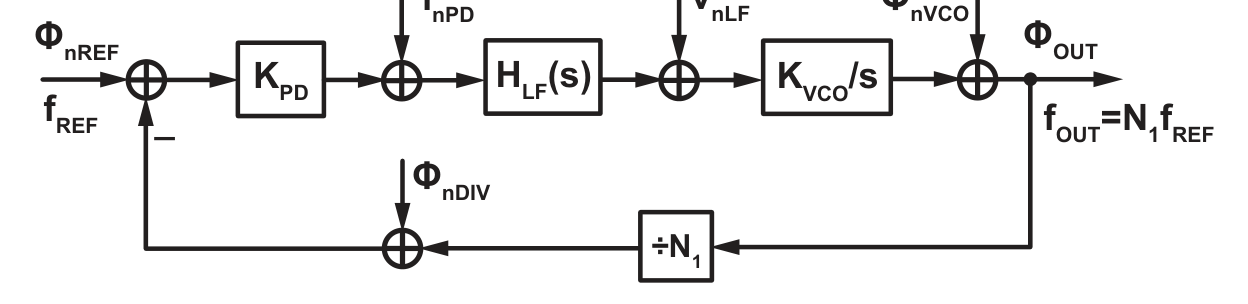
\includegraphics[keepaspectratio,width=0.85\columnwidth]{fig/fig_2_1.png}
  \caption{PLLの線形モデル(本文Fig.\,2.1，\cite{osada_thesis})．ループの各所(基準・PD・ループフィルタ・VCO・分周器)にそれぞれ固有の雑音源がぶら下がる形でモデル化できる．}
  \label{fig:pll-linear-model}
\end{figure}

PLLは負帰還系であるため，図\ref{fig:feedback-noise-amp}(a)に示すように単純化して記述できる．帰還利得を $\beta$ ，フィードフォワード利得を $A(s)$ とすると，ループ利得が十分大きい帯域($|\beta A(s)| \gg 1$，VCOの積分特性とPLLの追従動作により，通常はこの条件が満たされるように設計される)では，閉ループゲインは $\frac{A(s)}{1 + \beta A(s)} \approx \frac{1}{\beta}$ と近似できる．つまり，ループの入力側に入る雑音は，出力時に $1/\beta$ 倍に増幅されて現れるということである．従来型のPLLでは帰還経路に分周比 $N$ の分周器を用いるため $\beta = 1/N$ となり，基準発振器やPDの雑音，そして後述する分周器由来の(量子化)雑音は，すべて \textbf{$N$ 倍}に増幅されて出力に現れることになる(図\ref{fig:feedback-noise-amp}(b))．例えば基準周波数100\,MHzから2.4\,GHzを生成する場合，$N=24$ であるから $20\log_{10}(24) \approx 27.6$\,dBもの増幅を受ける．これが，分数分周比PLLを設計する上での根本的な制約となる．

\begin{figure}[H]
  \centering
  
\includegraphics[keepaspectratio,width=0.85\columnwidth]{fig/fig_3_1.png}
  \caption{負帰還系における入力換算雑音の増幅(本文Fig.\,3.1，\cite{osada_thesis})．(a)一般の負帰還系では入力側雑音は $1/\beta$ 倍される．(b)帰還を「割り算」(分周器，$\beta=1/N$)ではなく「引き算」(ミキサ，$\beta=1$)で実現すれば，雑音は増幅されない．それについては後述．}
  \label{fig:feedback-noise-amp}
\end{figure}

\subsection{分数分周比PLLにおける量子化雑音とフラクショナルスパー}

整数分周比のPLLに対し，出力周波数を基準周波数の小数倍に設定できる分数分周比(Fractional-$N$)PLLは，より細かい周波数分解能を実現できるため広く用いられている．分数分周は，マルチモジュラス分周器(Multi-Modulus Divider, MMD)の分周比を時間的に変化させ，その平均値として目的の小数分周比を実現する(例えば $\div 2.25$ を $2,3,2,2,\dots$ の繰り返しで近似する)．しかし瞬間の分周比は整数値をとり，その値が周期的に切り替わるため，位相誤差が常に変動する．これが\textbf{量子化雑音}であり，そのパターンが周期的だと鋭いスパー(フラクショナルスパー)として現れる．

この量子化雑音は，$\Delta\Sigma$変調器(Delta Sigma Modulator, DSM)によって高域へ押しやる「ノイズシェーピング」によってある程度緩和できる．これは，PLL自体がLPF特性を持つためである．しかし，それでも前述の閉ループゲイン $1/\beta = N$ による増幅を免れることはできない．結果として，分数分周比PLLは整数分周比PLLに比べ，量子化雑音の分だけジッタ性能が大きく悪化するという問題を抱えている(図\ref{fig:frac-pn})．

\begin{figure}[H]
  \centering
  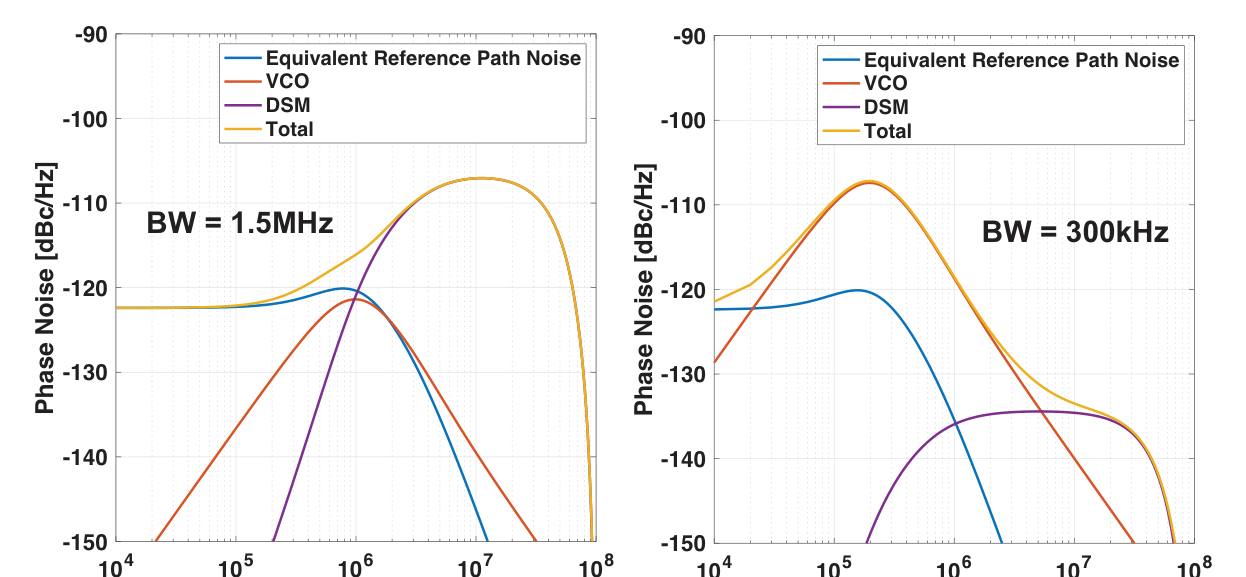
\includegraphics[keepaspectratio,width=0.85\columnwidth]{fig/fig_2_9.png}
  \caption{分数分周比PLLの位相雑音(本文Fig.\,2.9，\cite{osada_thesis})．量子化雑音が上乗せされ，帯域幅が1.5\,MHzでは高周波帯で量子化雑音が支配的になることが示されている．なお，狭帯域にしてもVCO雑音が増えるため根本解決にはならない．}
  \label{fig:frac-pn}
\end{figure}

\subsection{ノイズ増幅を回避する方法}

この量子化雑音増幅の問題に対し，近年注目されているアプローチの一つが，分周器を高調波ミキサ(Harmonic Mixer, HM)による周波数の「引き算」に置き換える方法である．ミキサによってHM出力 $f_\text{HM} = f_\text{OUT} - k f_\text{LO}$($k$ は高調波次数)を生成し，この信号を基準信号と比較する構成にする(ロック時には $f_\text{HM}=f_\text{REF}$ となる)．この時，除算は行われないため，閉ループゲインは $\beta \approx 1$(ユニティ)となり，量子化雑音は増幅されない．したがって，分数分周比PLLの課題である量子化雑音の増幅を回避できる．

なお，$k$倍せず直接$f_\text{HM} = f_\text{OUT} - f_\text{LO}$とすると，$f_\text{REF}$ は小さいため，$f_\text{OUT}$ と $f_\text{LO}$ が非常に近い周波数となる．この場合，その2つが相互に影響しあって新たなノイズを生み出すリスクが生じる．$k$倍することで，相互に影響する高調波成分を非常に弱めることができるため，このような構成が採用される．

% !TEX root = main.tex
\section{量子化雑音の抑制手法とフィードフォワード型構成}
\label{sec:methods}

\subsection{既存の量子化雑音抑制手法}

分数分周比PLLの量子化雑音を抑制する手法は，大きく以下の3系統に整理できる．

\begin{enumerate}
  \item \textbf{デジタル-時間変換器(Digital-to-Time Converter, DTC)等によるノイズキャンセル：} MMDの制御列から期待される位相誤差を予測し，DTCで基準経路の時間をずらすことでキャンセルする．しかし，DTCが作る遅延は，温度や電圧，製造のばらつきにより変動しやすい．したがって，そのずれをキャリブレーションする回路が必要となる．また，キャリブレーションの収束には数十\,$\mu$s ~ 数\,msの時間がかかるうえ，PLLの出力周波数を切り替える度に再度キャリブレーションが必要になる(DTCの動作点が変わるため)．よって，特に頻繁に周波数が切り替わる設計の場合，PLLの出力品質が悪い時間が長いという欠点がある．
  \item \textbf{ノイズシェーピング周波数を上げる：} DSMの動作周波数(基本構成では基準周波数 $f_\text{REF}$ に一致)を高めることで，量子化雑音をより高域に押しやり，狭いループ帯域でも十分に除去できるようにする．しかし，そのためには高い基準周波数を持つ水晶発振器が必要となるため，必要コストが増大する．
  \item \textbf{等価FIRフィルタによる追加フィルタリング：} 同じPLLの出力成分に，遅延だけを変えた経路を複数用意する．各経路から出力された電流を(重みを変えて)足し合わせ平均化することで，主信号成分はそのままに雑音のみをキャンセルすることができる．これは，PLL出力それ自体は遅延に関係なく同じ値に収束するのに対し，量子化雑音は経路ごとにタイミングがずれるためである．しかし，遅延線が複雑になることや，消費電力が増大することが欠点である．
\end{enumerate}

第\ref{sec:pll-basics}節で述べた，フィードバックパスを分周器から高調波ミキサによる「引き算」に置き換える手法は，これら3系統とは異なる「新しいつまみ」として近年注目されており，他の手法と組み合わせることも可能である．ただし，この構成では補助PLLが新たに必要となるため，その補助VCOの消費電力や雑音をいかに抑えるかが課題となる．

\subsection{フィードフォワード(FF)型構成}

この補助VCOの雑音を軽減する手法として，Zhang et al.\cite{zhang_ffnc_2025}は，電圧領域のフィードフォワード雑音キャンセル(Feed-Forward Noise Cancellation, FFNC)を提案している(図\ref{fig:ff-concept})．この手法は，補助PLL側のPD出力(＝補助VCOの位相雑音の情報を含む信号)を，そのまま主ループのPD出力に加算するというものである．補助PLLにおいては，補助VCOの雑音はフィードバックパスに入る．それに対し，主ループでは基準側に入る．この入力経路の違いにより，2つを足し合わせることでノイズを打ち消すことができるのである．この手法は，補助PLLの雑音を打ち消すために高速な遅延線(VCDL)を用いる必要がなく，消費電力を抑えられるという利点がある．

\begin{figure}[H]
  \centering
  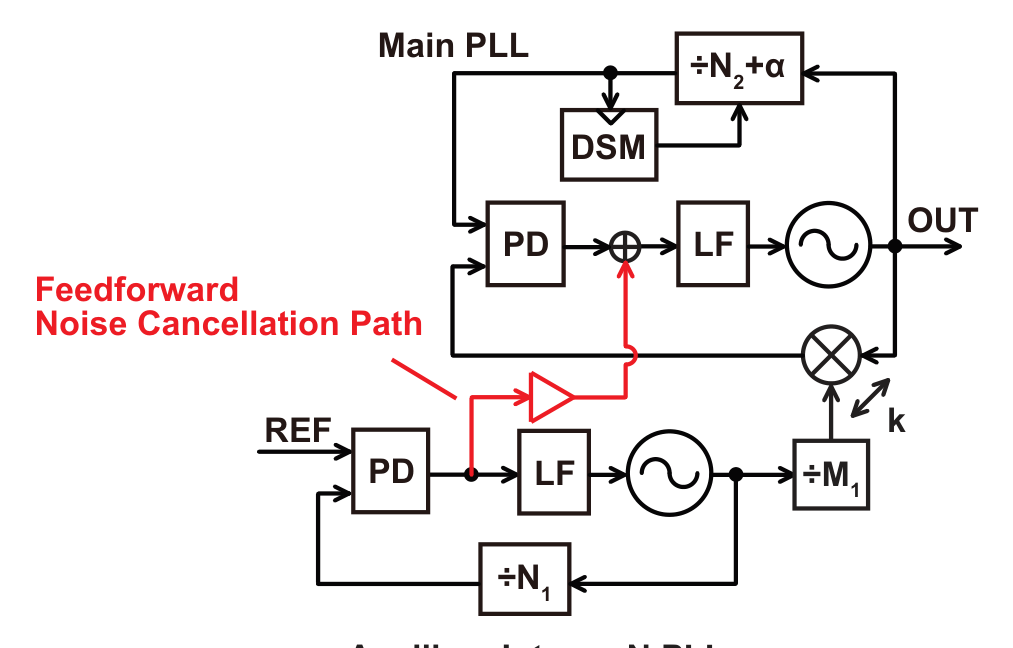
\includegraphics[keepaspectratio,width=0.85\columnwidth]{fig/fig_6_5.png}
  \caption{フィードフォワード雑音キャンセルの基本概念(本文Fig.\,6.5，\cite{osada_thesis})．補助PLLのPD出力を，電圧のまま主ループのPD出力に足し込むことで，高速な遅延線(VCDL)を使わずに補助VCOの雑音成分を打ち消す(\cite{zhang_ffnc_2025}, \cite{osada_thesis})．}
  \label{fig:ff-concept}
\end{figure}

\section{位相雑音抑制手法の概観とフィードフォワード型構成}
\label{sec:methods}

\subsection{既存の量子化雑音抑制手法}

分数分周比PLLの量子化雑音を抑制する手法は，大きく以下の3系統に整理できる．

\begin{enumerate}
  \item \textbf{デジタル-時間変換器（DTC）等によるノイズキャンセル：} MMDの制御列から期待される位相誤差を予測し，DTCで基準経路の時間をずらすことでキャンセルする．ジッタ・電力性能は優れるが，DTCの利得・線形性がプロセス・電圧・温度（PVT）変動の影響を強く受けるため，LMS等のキャリブレーションが必須であり，周波数切替のたびに数十\,$\mu$s〜数\,ms程度の収束時間を要する．
  \item \textbf{ノイズシェーピング周波数を上げる：} DSMの動作周波数（基本構成では基準周波数 $f_\text{REF}$ に一致）を高めることで，量子化雑音をより高域に押しやり，狭いループ帯域でも十分に除去できるようにする．高い基準周波数を得るための逓倍回路が別途必要になる．
  \item \textbf{等価FIRフィルタによる追加フィルタリング：} 主ループの帯域特性は変えずに，遅延の異なる複数の帰還信号を重み付き加算することで量子化雑音だけを追加的に整形する．経路間のゲイン・線形性のマッチングや遅延線の消費電力が課題となる．
\end{enumerate}

第\ref{sec:pll-basics}節で述べた，帰還を高調波ミキサによる「引き算」に置き換える手法（HMベース帰還）は，これら3系統とは異なる「新しいつまみ」として近年注目されており，他の手法と組み合わせることも可能である．

\subsection{HMベースPLLにおける補助PLLのオーバーヘッド}

HMベース帰還を用いるPLL（Dual-Feedback PLLなど）は，量子化雑音の増幅を回避できる一方，HM用の局部発振信号を生成する補助PLLが新たに必要になる．この補助PLLに含まれるVCOの位相雑音は，主ループの外側から加わる雑音源として出力に漏れ込むため，量子化雑音を抑えた代わりに補助VCOの雑音・消費電力のオーバーヘッドが新たな課題として生じる．

\subsection{最近提案されたフィードフォワード（FF）型構成}

この補助VCOのオーバーヘッドを軽減する手法として，Zhangら\cite{zhang_ffnc_2025}は電圧領域のフィードフォワード雑音キャンセル（Feed-Forward Noise Cancellation, FFNC）を提案している．この手法は，補助PLL側のPD出力（＝補助VCOの位相雑音の情報を含む信号）を，そのまま主ループのPD出力に加算するというものである．時間領域で位相を補正する高速遅延線（VCDL）を必要とせず，カスケード接続された2段目のPD出力の時点で信号がすでに低周波の電圧領域に落ちていることを利用して，低速なアンプと抵抗加算のみでキャンセルを実現している点が特徴である．65\,nm CMOSで試作した結果，106\,fs$_\mathrm{rms}$のジッタと$-63$\,dBcの最悪フラクショナルスパーを達成し，キャリブレーション不要という利点を保ったまま最先端級の性能を実証している．

\begin{figure}[H]
  \centering
  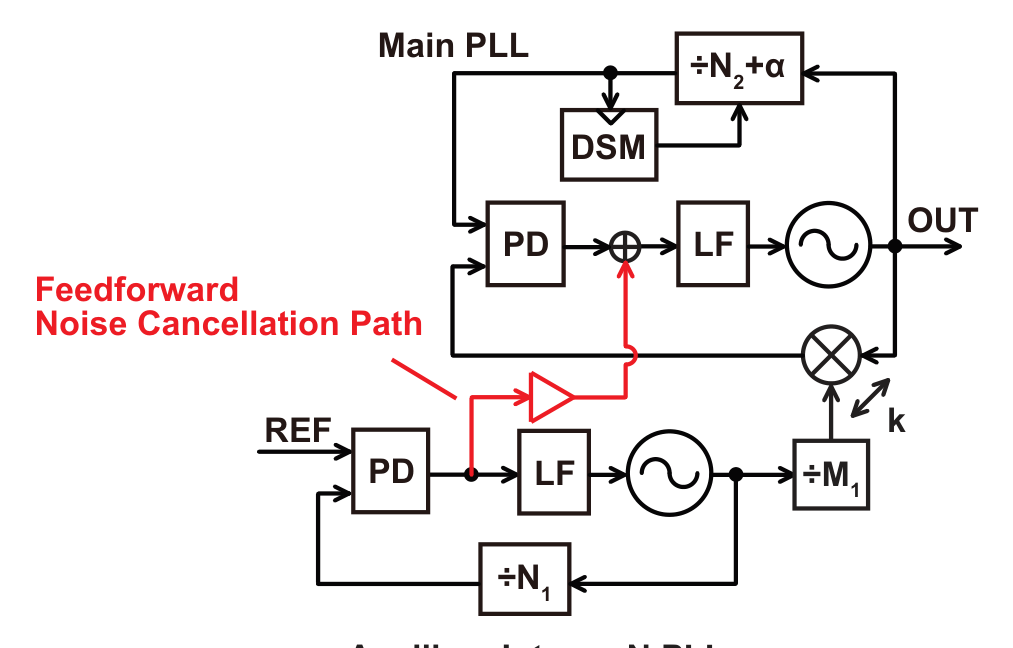
\includegraphics[keepaspectratio,width=0.85\columnwidth]{fig/fig_6_5.png}
  \caption{フィードフォワード雑音キャンセルの基本概念．補助PLLのPD出力を，電圧のまま主ループのPD出力に足し込むことで，高速な遅延線を使わずに補助VCOの雑音成分を打ち消す（\cite{zhang_ffnc_2025}, \cite{osada_thesis}第6章）．}
  \label{fig:ff-concept}
\end{figure}

% 9/17MTGまでは5~7章(提案・実績・Future Work)は未着手のまま持っていく方針のためコメントアウト(9/17以降に戻す)
% % !TEX root = main.tex
\section{提案：最適化フレームワークへのフィードフォワード型構成の導入}
\label{sec:proposal}

\subsection{既存の最適化フレームワーク}

本研究室では，PLLのジッタと消費電力の間のトレードオフを定量的に比較するための最適化フレームワークが提案されている\cite{zhu_moea_2025}．このフレームワークは，多目的進化アルゴリズム（Multi-Objective Evolutionary Algorithm, MOEA，具体的にはNSGA-II）を用いて，PLLの各ブロックの消費電力やループ帯域周波数などを決定変数として探索し，積分ジッタとトータル消費電力の2つの目的関数について，一方を改善すればもう一方が悪化するという意味で最適な解の集合（パレートフロント）を求めるものである．これにより，従来は設計者が数式変形と勘に頼って行っていたジッタ・電力トレードオフの評価を，体系的かつ網羅的に行うことができる．

このフレームワークは，従来型の整数分周比PLL，DTCベースPLL，およびHMベースのDual-Feedback PLLを対象に，ジッタ・電力のパレートフロントを比較しており，各アーキテクチャがどのような条件で優位に立つかを議論している．しかし，第\ref{sec:methods}節で述べたフィードフォワード型構成は，このフレームワークにはまだ組み込まれていない．

\subsection{本研究で行うこと}

そこで本研究では，この最適化フレームワークに，フィードフォワード型構成のノイズ伝達関数を新たに組み込む．具体的には，補助PLLの雑音源から出力までの伝達関数に，フィードフォワードによるキャンセル項（ゲイン整合条件を含む）を追加したモデルを構築し，これを目的関数（積分ジッタ・消費電力）の計算に反映させる．

これにより，(1)DTCベースPLL，(2)フィードフォワードなしのHMベースDual-Feedback PLL，(3)フィードフォワード型構成を備えたDual-Feedback PLL，の3アーキテクチャについて，同一の枠組みの上でジッタ・電力パレートフロントを比較することが可能になる．この比較を通じて，フィードフォワード型構成がどのジッタ・電力の領域で他の構成に対して優位に立つのかを明らかにすることが，本研究の中心的な取り組みである．

% \include{section6}
% \section{これまでの成果}
\label{sec:progress}

本研究は現時点では新規の回路提案や測定を行う段階には至っておらず，第\ref{sec:proposal}節で述べた比較検討を行うための土台を整備する段階にある．これまでに行った作業は，大きく以下の2点である．

\subsection{既存最適化プログラムの再現}

まず，先輩から提供を受けたMATLABプログラム（NSGA-IIに基づく多目的最適化フレームワーク\cite{zhu_moea_2025}の実装）を実行し，論文中と同様のジッタ・電力パレートフロントが得られることを確認した．図\ref{fig:pareto-compare}に，DTCベースPLLとHMベースDual-Feedback PLLのジッタ・電力トレードオフを比較したパレートフロントを，図\ref{fig:pareto-final}に最適化計算の最終結果の一例を示す．いずれも先輩のプログラムをそのまま実行して得たものであり，フレームワークの動作を自身の手元で確認できたことを意味する。

\begin{figure}[H]
  \centering
  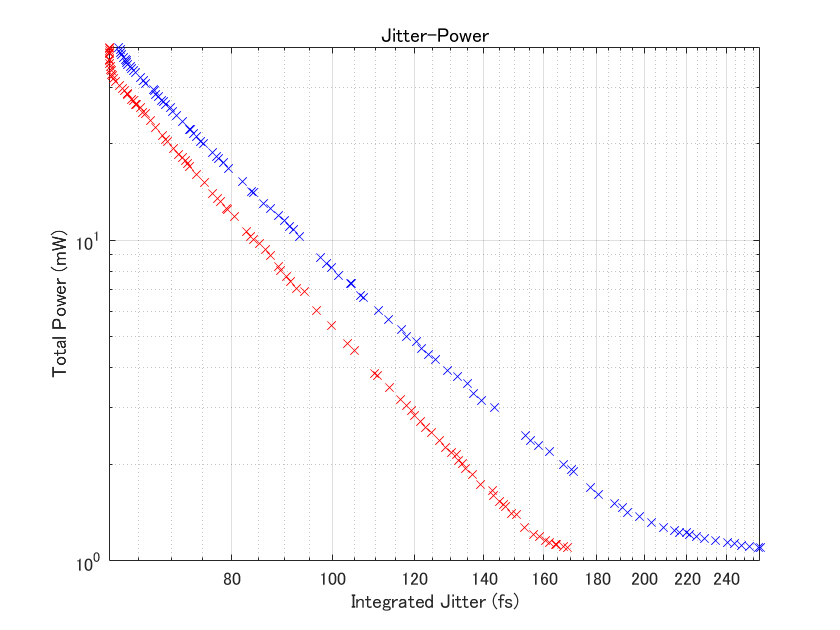
\includegraphics[keepaspectratio,width=0.8\columnwidth]{fig/matlab_pareto_compare.png}
  \caption{既存プログラムによるジッタ・電力パレートフロントの再現例（2アーキテクチャの比較）．}
  \label{fig:pareto-compare}
\end{figure}

\begin{figure}[H]
  \centering
  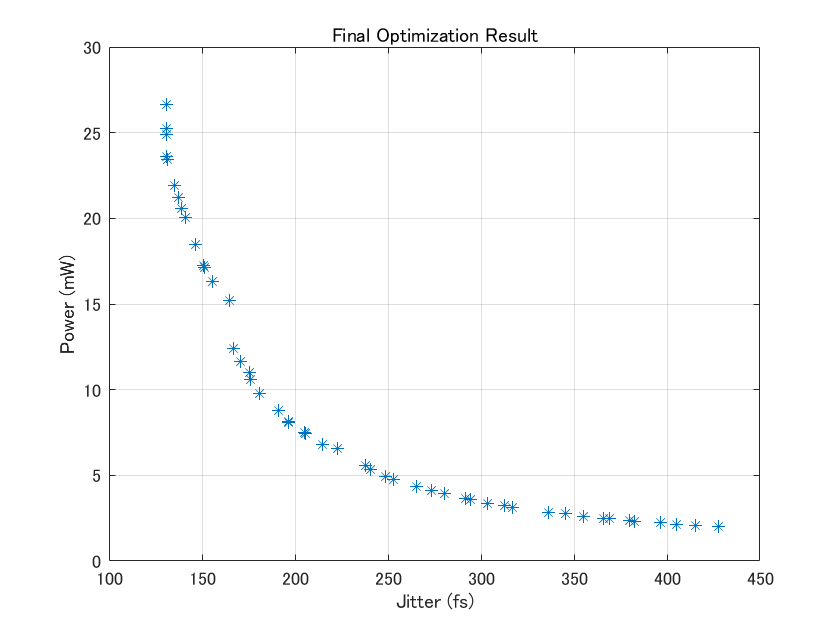
\includegraphics[keepaspectratio,width=0.8\columnwidth]{fig/matlab_pareto_final.png}
  \caption{NSGA-IIによる最適化計算の最終世代の結果例（ジッタ vs 消費電力）．}
  \label{fig:pareto-final}
\end{figure}

\subsection{フィードフォワード型構成の理解とモデル化に向けた準備}

次に，第\ref{sec:methods}節で紹介したフィードフォワード型構成\cite{zhang_ffnc_2025}の技術内容の理解を進めた．位相検出器のゲインやループフィルタの伝達関数（原論文の式(6)・式(7)に相当する部分）については，導出過程を自分の手で追い直し，内容を確認できた．一方で，補助PLLから出力までの伝達関数（原論文の式(8)以降，フィードフォワードによるキャンセル項を含む部分）については，式の導出過程に理解が及んでいない箇所が残っており，この部分をノイズ解析モデルへ正確に反映するところまでは至っていない。

並行して，Dual-Feedback構成において，補助（外部）PLLの雑音寄与を主ループの雑音源（基準・PD・ループフィルタ・VCO・DSM量子化雑音）から分離し，それぞれの積分ジッタへの寄与率を算出できるMATLABモデル（\texttt{DualFF\_typeI\_typeII\_lag\_lead\_lag.m}）を構築した。ただし，このモデルは現時点ではフィードフォワードによるキャンセル項を含んでおらず，キャンセルを行わない状態での補助PLL寄与を可視化するにとどまっている。

% TODO: DualFF_typeI_typeII_lag_lead_lag.m を実行して得られる位相雑音特性カーブ（figure 1, figure 2：補助ループ・主ループそれぞれのノイズ寄与内訳）をここに貼る。
% \begin{figure}[H]
%   \centering
%   \includegraphics[keepaspectratio,width=0.8\columnwidth]{fig/dualff_phase_noise.png}
%   \caption{補助PLLの雑音寄与を分離したノイズ解析モデルの出力例．}
%   \label{fig:dualff-pn}
% \end{figure}

フィードフォワード型構成のジッタ・電力への効果を定量的に評価するには，このキャンセル項をモデルに導入する必要があり，これが直近の課題である（第\ref{sec:future}節）。


\bibliographystyle{junsrt}
\bibliography{cite}

\end{document}
